\documentclass{beamer}
\usetheme[sectionpage=none, progressbar=frametitle, numbering=none]{metropolis}        % Use metropolis theme
\usepackage{tikz}
\usetikzlibrary{tikzmark,decorations.pathreplacing,calc}
\usepackage{listings}
\title{An Architecture for Task and Traffic Offloading in Edge Computing via Deep Learning}
%\date{\today}
\date{April 9, 2018}
\author{Alessandro Gaballo}
\institute{Supervisor: Flavio Esposito - Saint Louis University\\
			Cosupervisor: Guido Marchetto - Politecnico di Torino}

\setbeamertemplate{frametitle continuation}{\insertcontinuationcount}
% logo of my university
\titlegraphic{%
  \begin{picture}(0,0)
    \put(283,-145){\makebox(0,0)[rt]{
\includegraphics[width=1.5cm]{img/politologo}}}
    \put(290,-120){\makebox(0,0)[rt]{
\includegraphics[width=2cm]{img/slulogo1}}}

  \end{picture}} 
 
\AtBeginSection[]{
%\frame{\sectionpage}
}

\newcommand{\mytoc}{\frame{\frametitle{Talk overview}\tableofcontents[currentsection,currentsubsection,subsectionstyle=show/shaded/hide, subsubsectionstyle=show/shaded/hide]}}



%subsubsection page
\newcommand{\subsubsectionpage}{
\begin{frame}
  \centering
  \begin{minipage}{22em}
    \raggedright
    \usebeamercolor[fg]{section title}
    \usebeamerfont{section title}
    \insertsectionhead\\[-1ex]
    \usebeamertemplate*{progress bar in section page}
    \par
    \ifx\insertsubsectionhead\@empty\else%
      \usebeamercolor[fg]{subsection title}%
      \usebeamerfont{subsection title}%
      \insertsubsectionhead{} -- \insertsubsubsectionhead
    \fi
  \end{minipage}
  \par
  \vspace{\baselineskip}
\end{frame}
}

\newcommand\blfootnote[1]{%
  \begingroup
  \renewcommand\thefootnote{}\footnote{#1}%
  \addtocounter{footnote}{-1}%
  \endgroup
}

% reshaping list circles bullet
\setbeamertemplate{section in toc}{\leavevmode\leftskip=2ex%
  \llap{%
    \usebeamerfont*{section number projected}%
    \usebeamercolor{section number projected}%
    \begin{pgfpicture}{-1ex}{0ex}{1ex}{2ex}
      \color{bg}
      \pgfpathcircle{\pgfpoint{0pt}{.75ex}}{.6ex}
      \pgfusepath{fill}
      %\pgftext[base]{\color{fg}\inserttocsectionnumber}
    \end{pgfpicture}\kern1.25ex%
  }%
  \inserttocsection\par}
  
\setbeamertemplate{subsection in toc}{\leavevmode\leftskip=1em$\bullet$\hskip1em\inserttocsubsection\par}
\setbeamertemplate{subsubsection in toc}{\leavevmode\leftskip=3em$\bullet$\hskip1em\inserttocsubsubsection\par}

%temporary until I remake the imgs
\setbeamercolor{background canvas}{bg=white}

\definecolor{colori}{RGB}{166,35,41}
\definecolor{colorii}{RGB}{248,219,162}


\begin{document}
\maketitle
\section*{Motivation}
  \begin{frame}{How many times have you delegated a task?}
	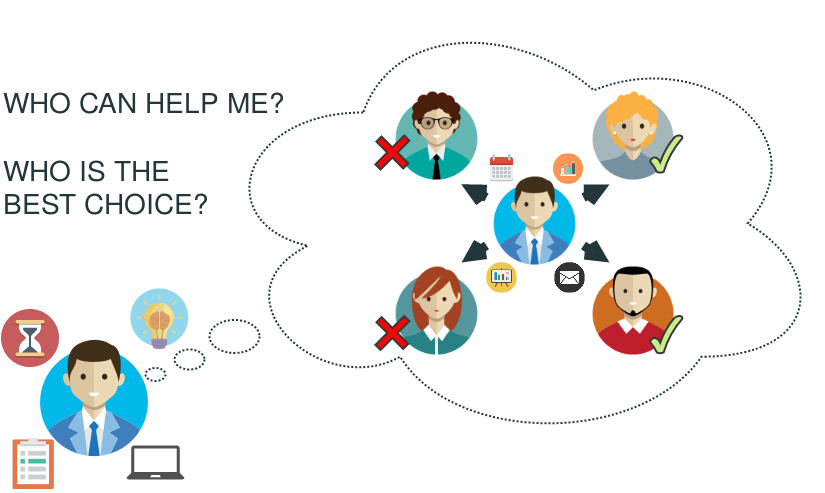
\includegraphics[width=\textwidth]{img/delegation}  
  \end{frame}
  
  \frame{\frametitle{What is task offloading and how should it be done?}
  	\begin{columns}[totalwidth=\textwidth]
	\begin{column}{0.65\textwidth}
	  Task offloading is the process of transferring tasks to another platform. \\~\\
	  There is no architecture describing the offloading mechanisms.\\~\\
	  Currently used routing strategies, such as OSPF, are performance unaware.
	\end{column}
	\begin{column}{0.33\textwidth}
	\centering	
	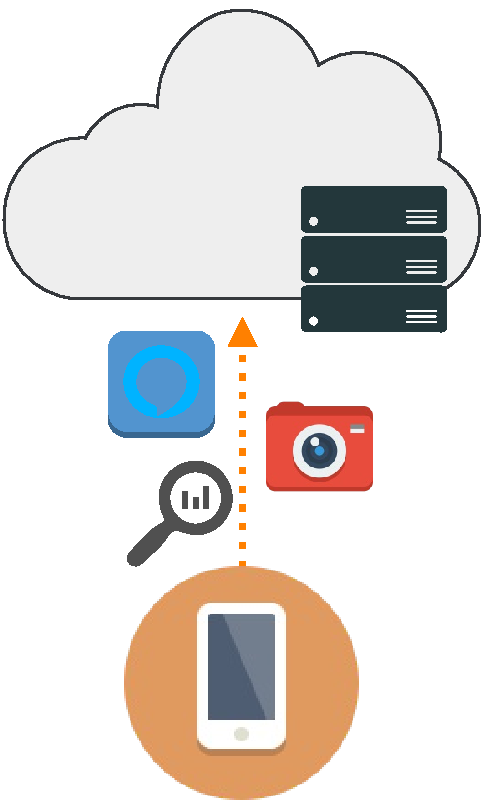
\includegraphics[scale=0.4]{img/offloading.pdf}
	\end{column}
	\end{columns}
  }

  
  \frame{\frametitle{What tools do we have and what can we do?}
	Recently the ideas of Software-Defined Networking (SDN) and Knowledge-Defined Networking (KDN)~[1] have spreaded.\\~\\

	The combination of SDN \& KDN represents a powerful tool for network management.\\~\\
	
	In this work we design a task offloading architecture to address the complexity problem and leverage a network knowledge plane to support performance aware traffic steering. \\~\\~\\
	 \begin{columns}[totalwidth=\textwidth]
	\begin{column}{0.35\textwidth}
	~
	\end{column}
	\begin{column}{0.63\textwidth}
	
	\scriptsize{[1] D. Clark, C. Partridge, J. Ramming, and J. Wroclawski. \\
	\textbf{A knowledge plane for the internet.} \\
	In Proc. of SIGCOMM '03. ACM, New York, NY, USA, 3-10.}
	\end{column}
	\end{columns}
  }
\begin{frame}{Talk overview}
	\tableofcontents[hideallsubsections]
\end{frame}
\section{Offloading Architecture}
\subsection{Architecture}
	\mytoc
	\begin{frame}{Our contribution: offloading architecture}
		\centering
		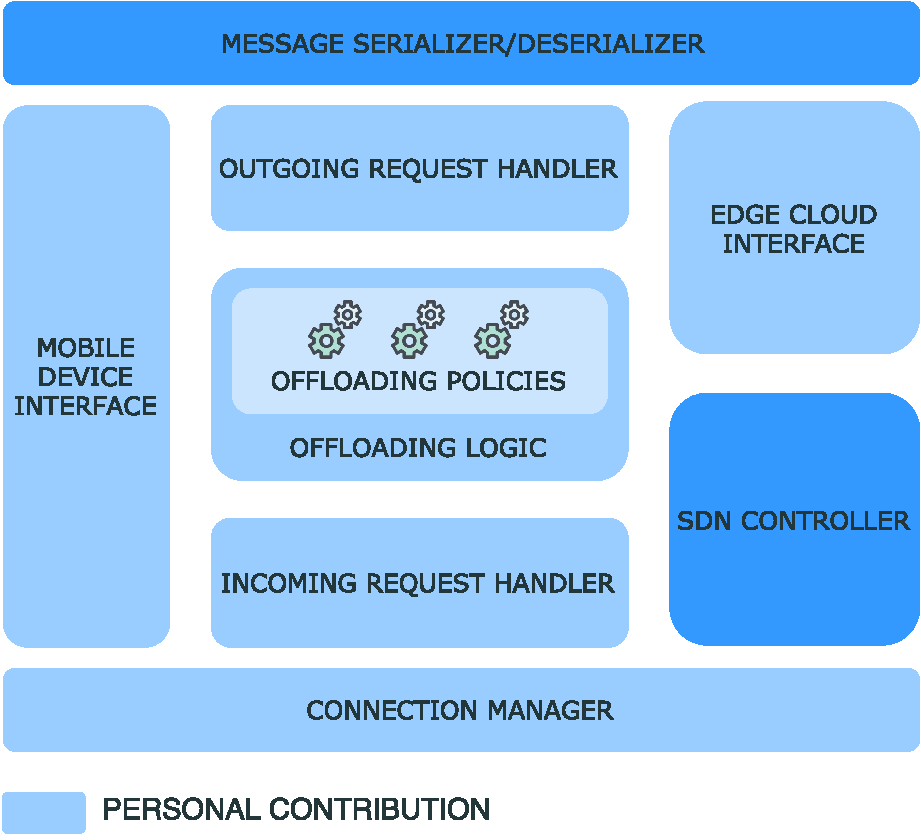
\includegraphics[scale=0.5]{img/off_sys_arch.pdf}
	\end{frame}

\subsection{Task Offloading Protocol}
	\mytoc
	\begin{frame}{Our contribution: task offloading protocol}
		\centering
		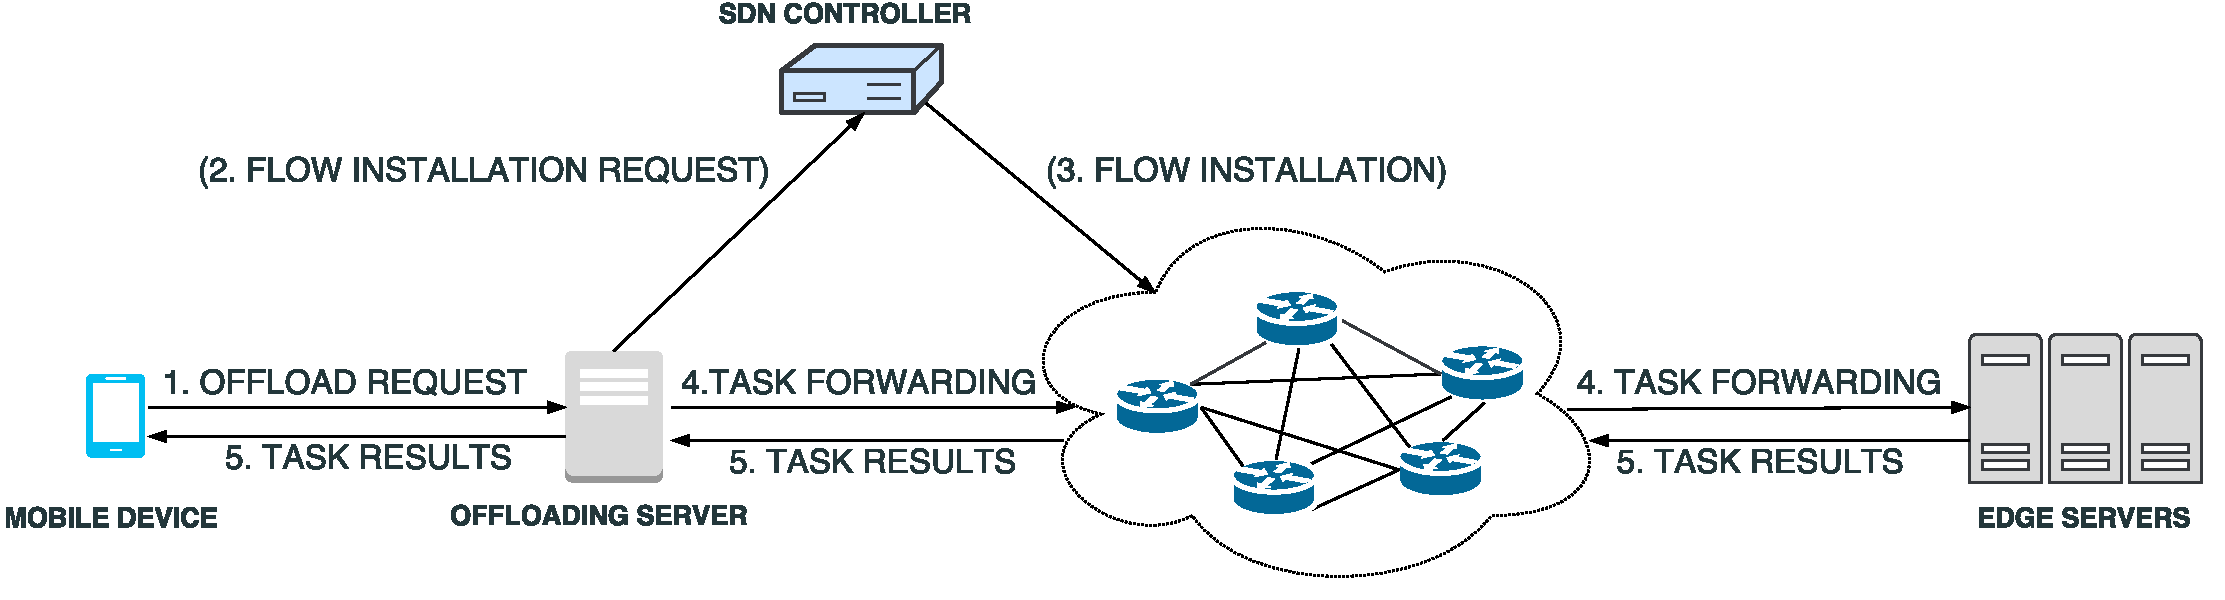
\includegraphics[scale=0.3]{img/protocol_sequence.pdf}
		\flushleft
		The protocol allows the client to specify:
		\begin{itemize}
		\item task requirements such as CPU, memory and latency
		\item offloading logic (e.g. nearest server)
		\end{itemize}
	\end{frame}

\subsection{Path Prediction via Deep Learning}	
	\mytoc
	\begin{frame}{Our contribution: path prediction via deep learning}
	Deep learning is a powerful tool for inference tasks
	\\~\\
	\centering	
	{\Huge$\Downarrow$}
	\flushleft
	\textbf{IDEA:} Routing problem as inference problem
	\end{frame}
	
	\frame{\frametitle{Long Short-Term Memory (LSTM)}
	LSTM is an evolution of recurrent neural networks (RNNs) capable of memorizing data temporal patterns\\~\\
	\textbf{Objective:}\\Learn how traffic patterns evolve and route accordingly
	}
	\frame{\frametitle{Learning from who?}LSTM RNNs  are a supervised learning method, they require data to learn from.\\ 
	We use OSPF routing decisions as a ground truth.\\~\\
	\centering
	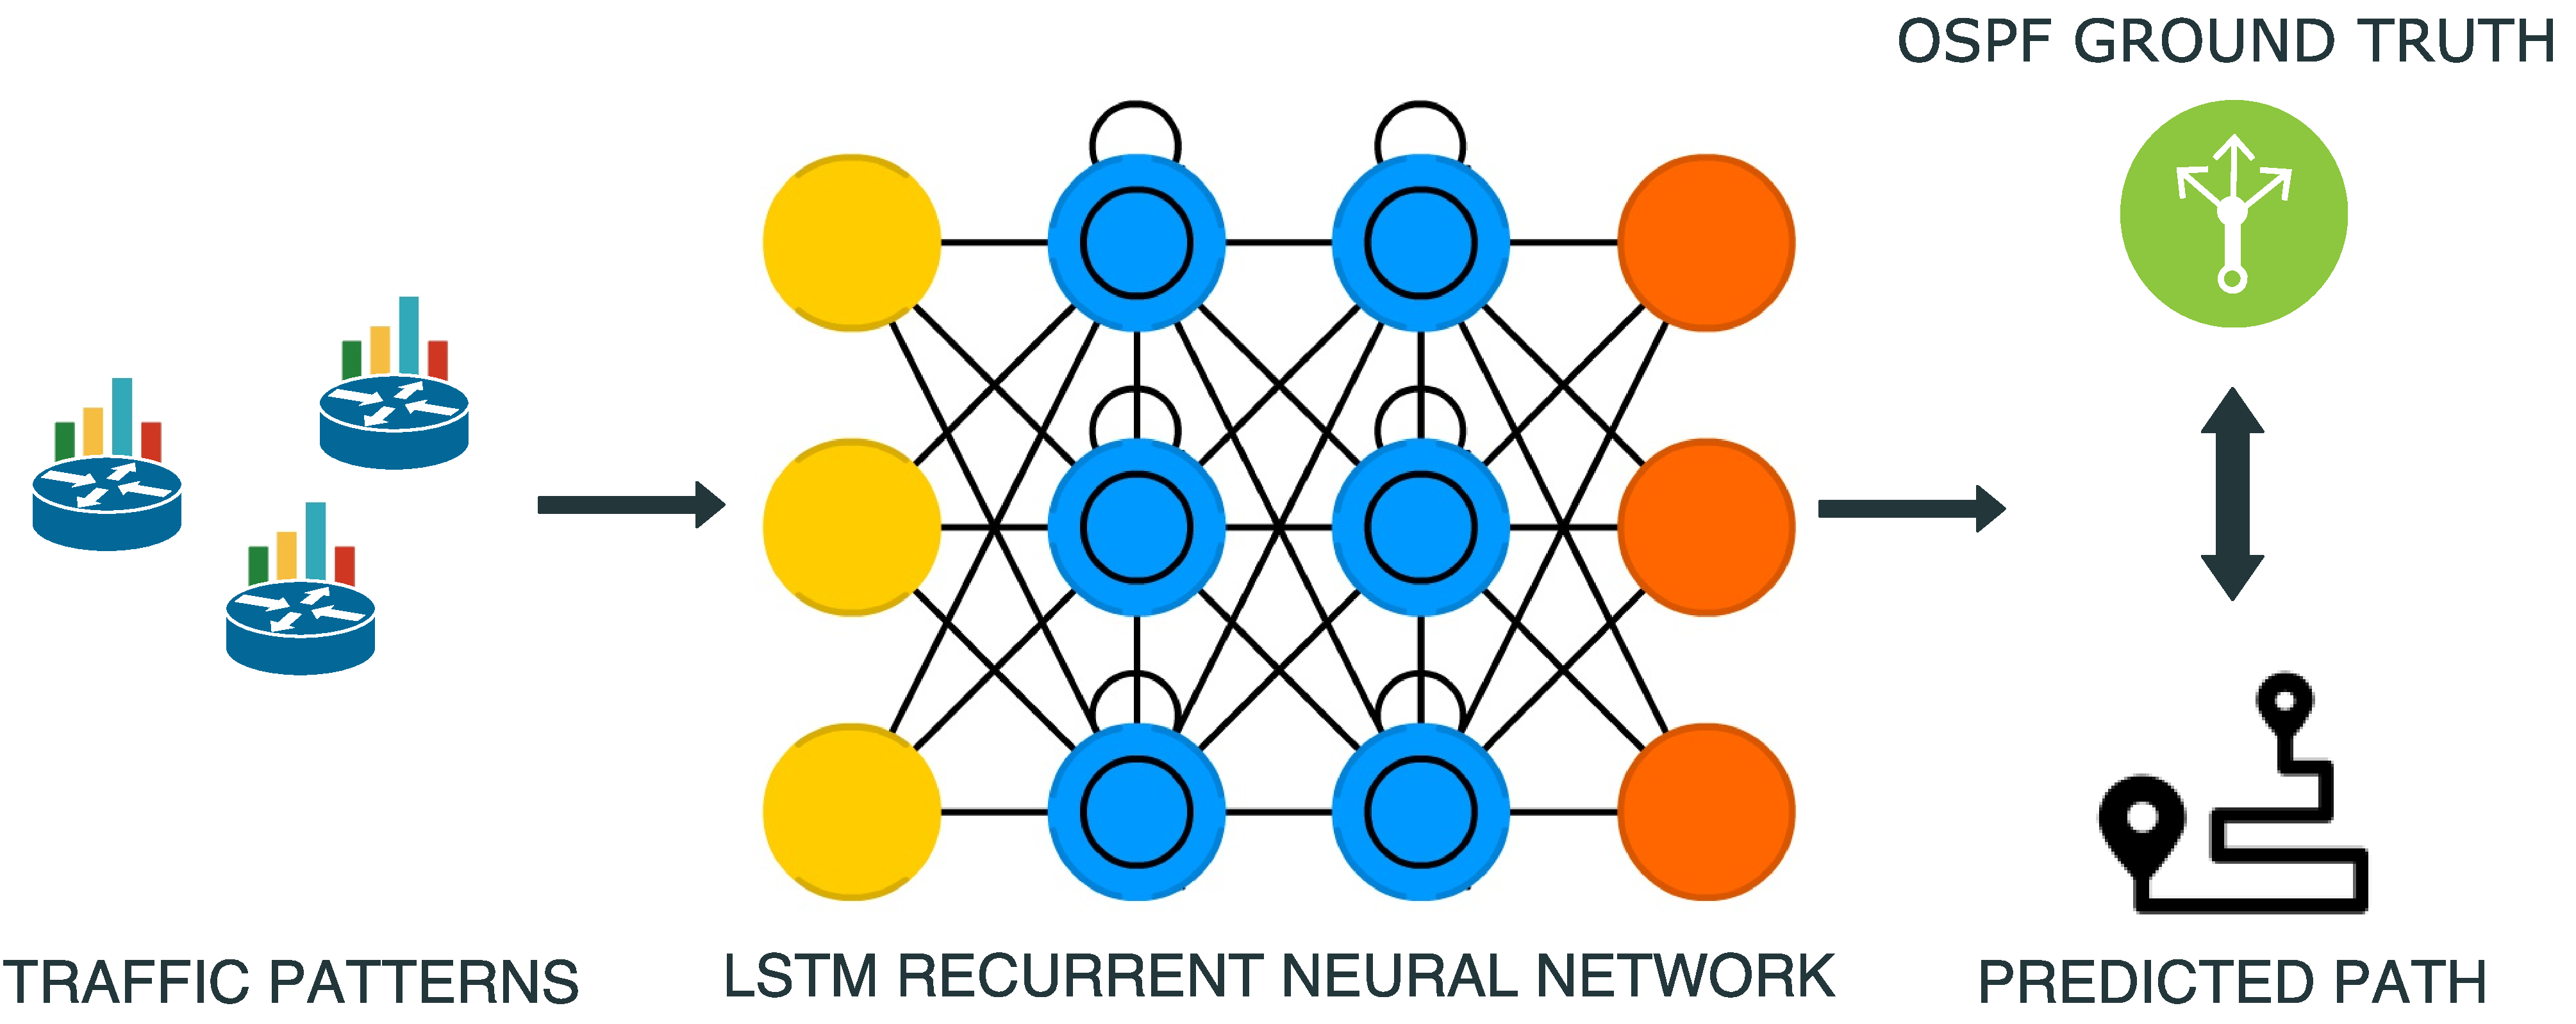
\includegraphics[width=\textwidth]{img/problem_model}
	}
	
\section{Results}
	\subsection{LSTM architecture}
	\mytoc

	\frame{\frametitle{Accuracy: more neurons or more layers?}
	Neurons affect performance more than hidden layers\\~\\	
	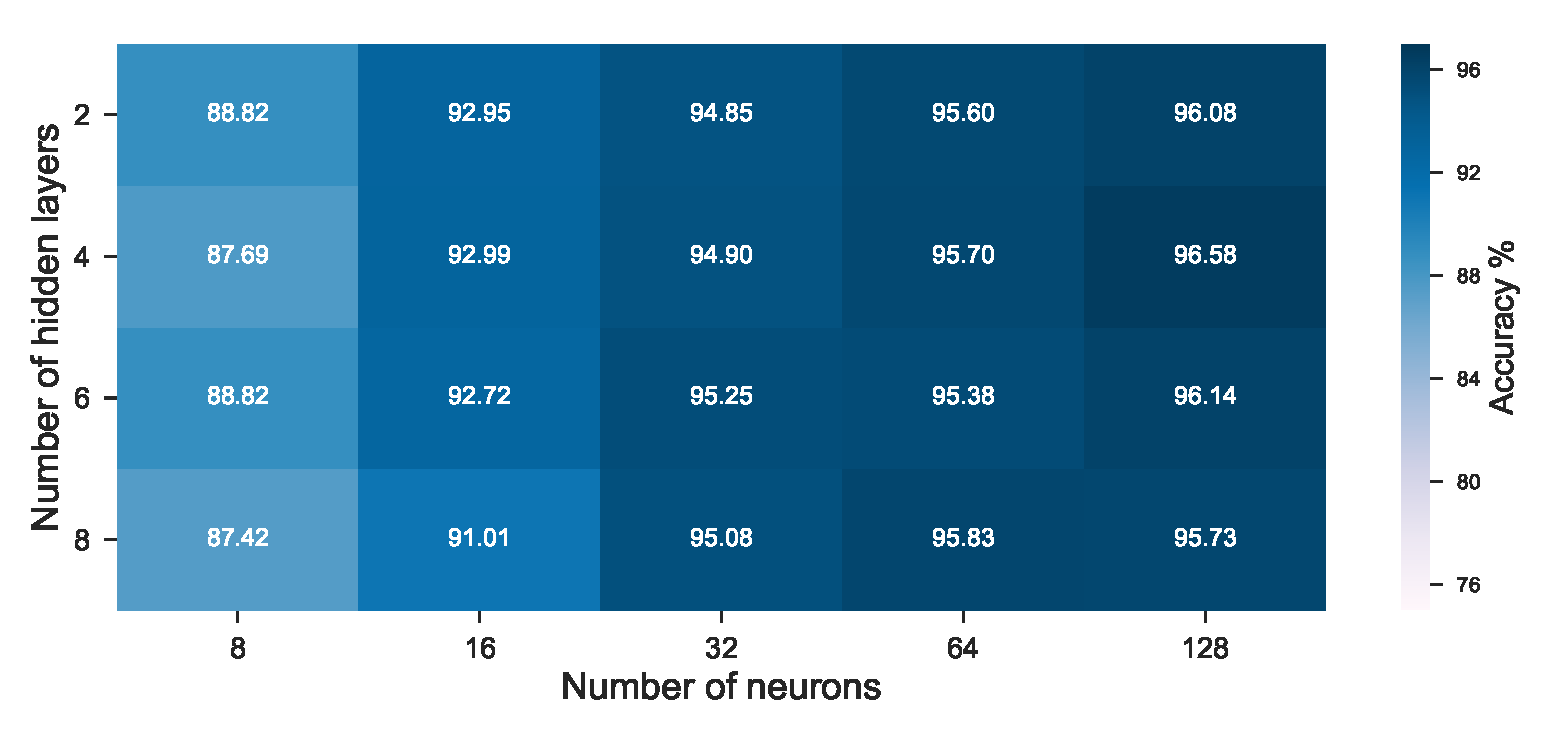
\includegraphics[width=\textwidth]{img/architecture_cmp}	
	}
	
	\frame{\frametitle{Finding the trade-off: training time}
	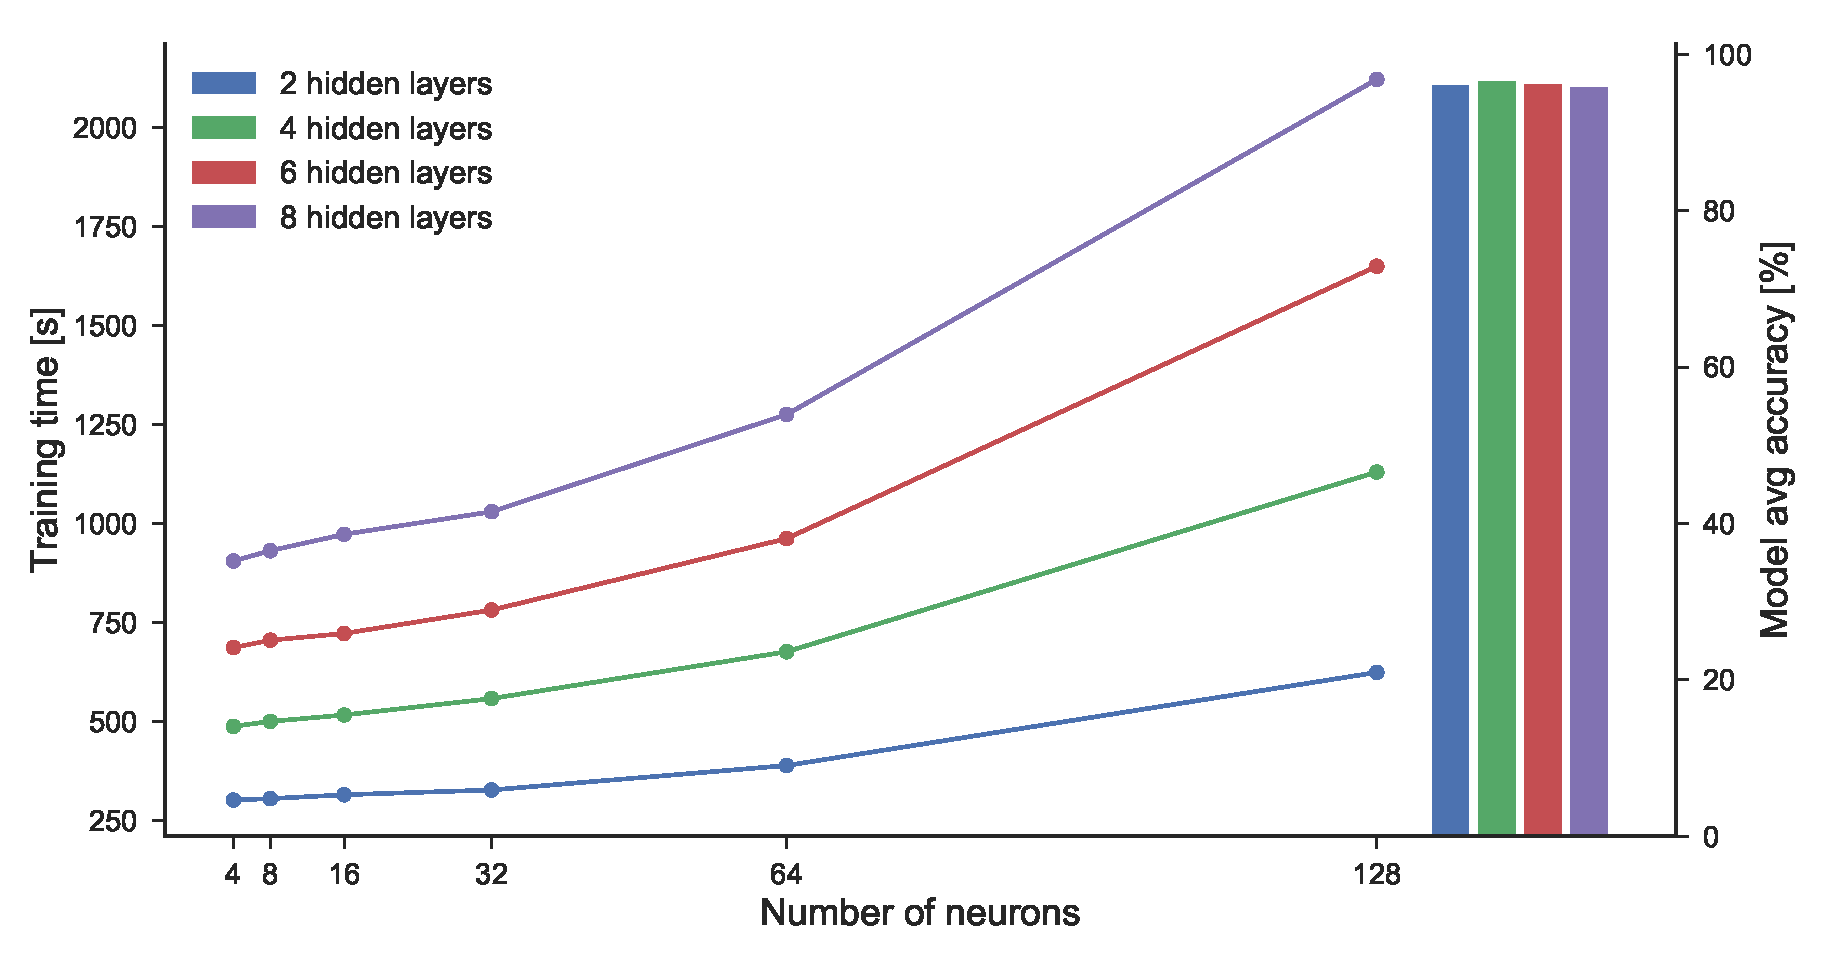
\includegraphics[width=\textwidth]{img/timing_cmp}	\\~\\
	\tiny{\textit{* Accuracy shown only for models with 128 neurons}}	
	}

	
	\subsection{Emulating OSPF}
	\mytoc
	\frame{\frametitle{The system is able to emulate OSPF}
	We test the system's ability to behave like OSPF by averaging the performance of all the models on the test set.\\~\\The LSTM achieves an average accuracy of \textbf{98.71\%} with respect to OSPF.}

	\subsection{Performance aware routing}
	\mytoc
	\frame{\frametitle{The LSTM system exhibits a dynamic behavior}
	We select a target and analyze how our system behaves differently from OSPF in case of link loss
	
	\centering
	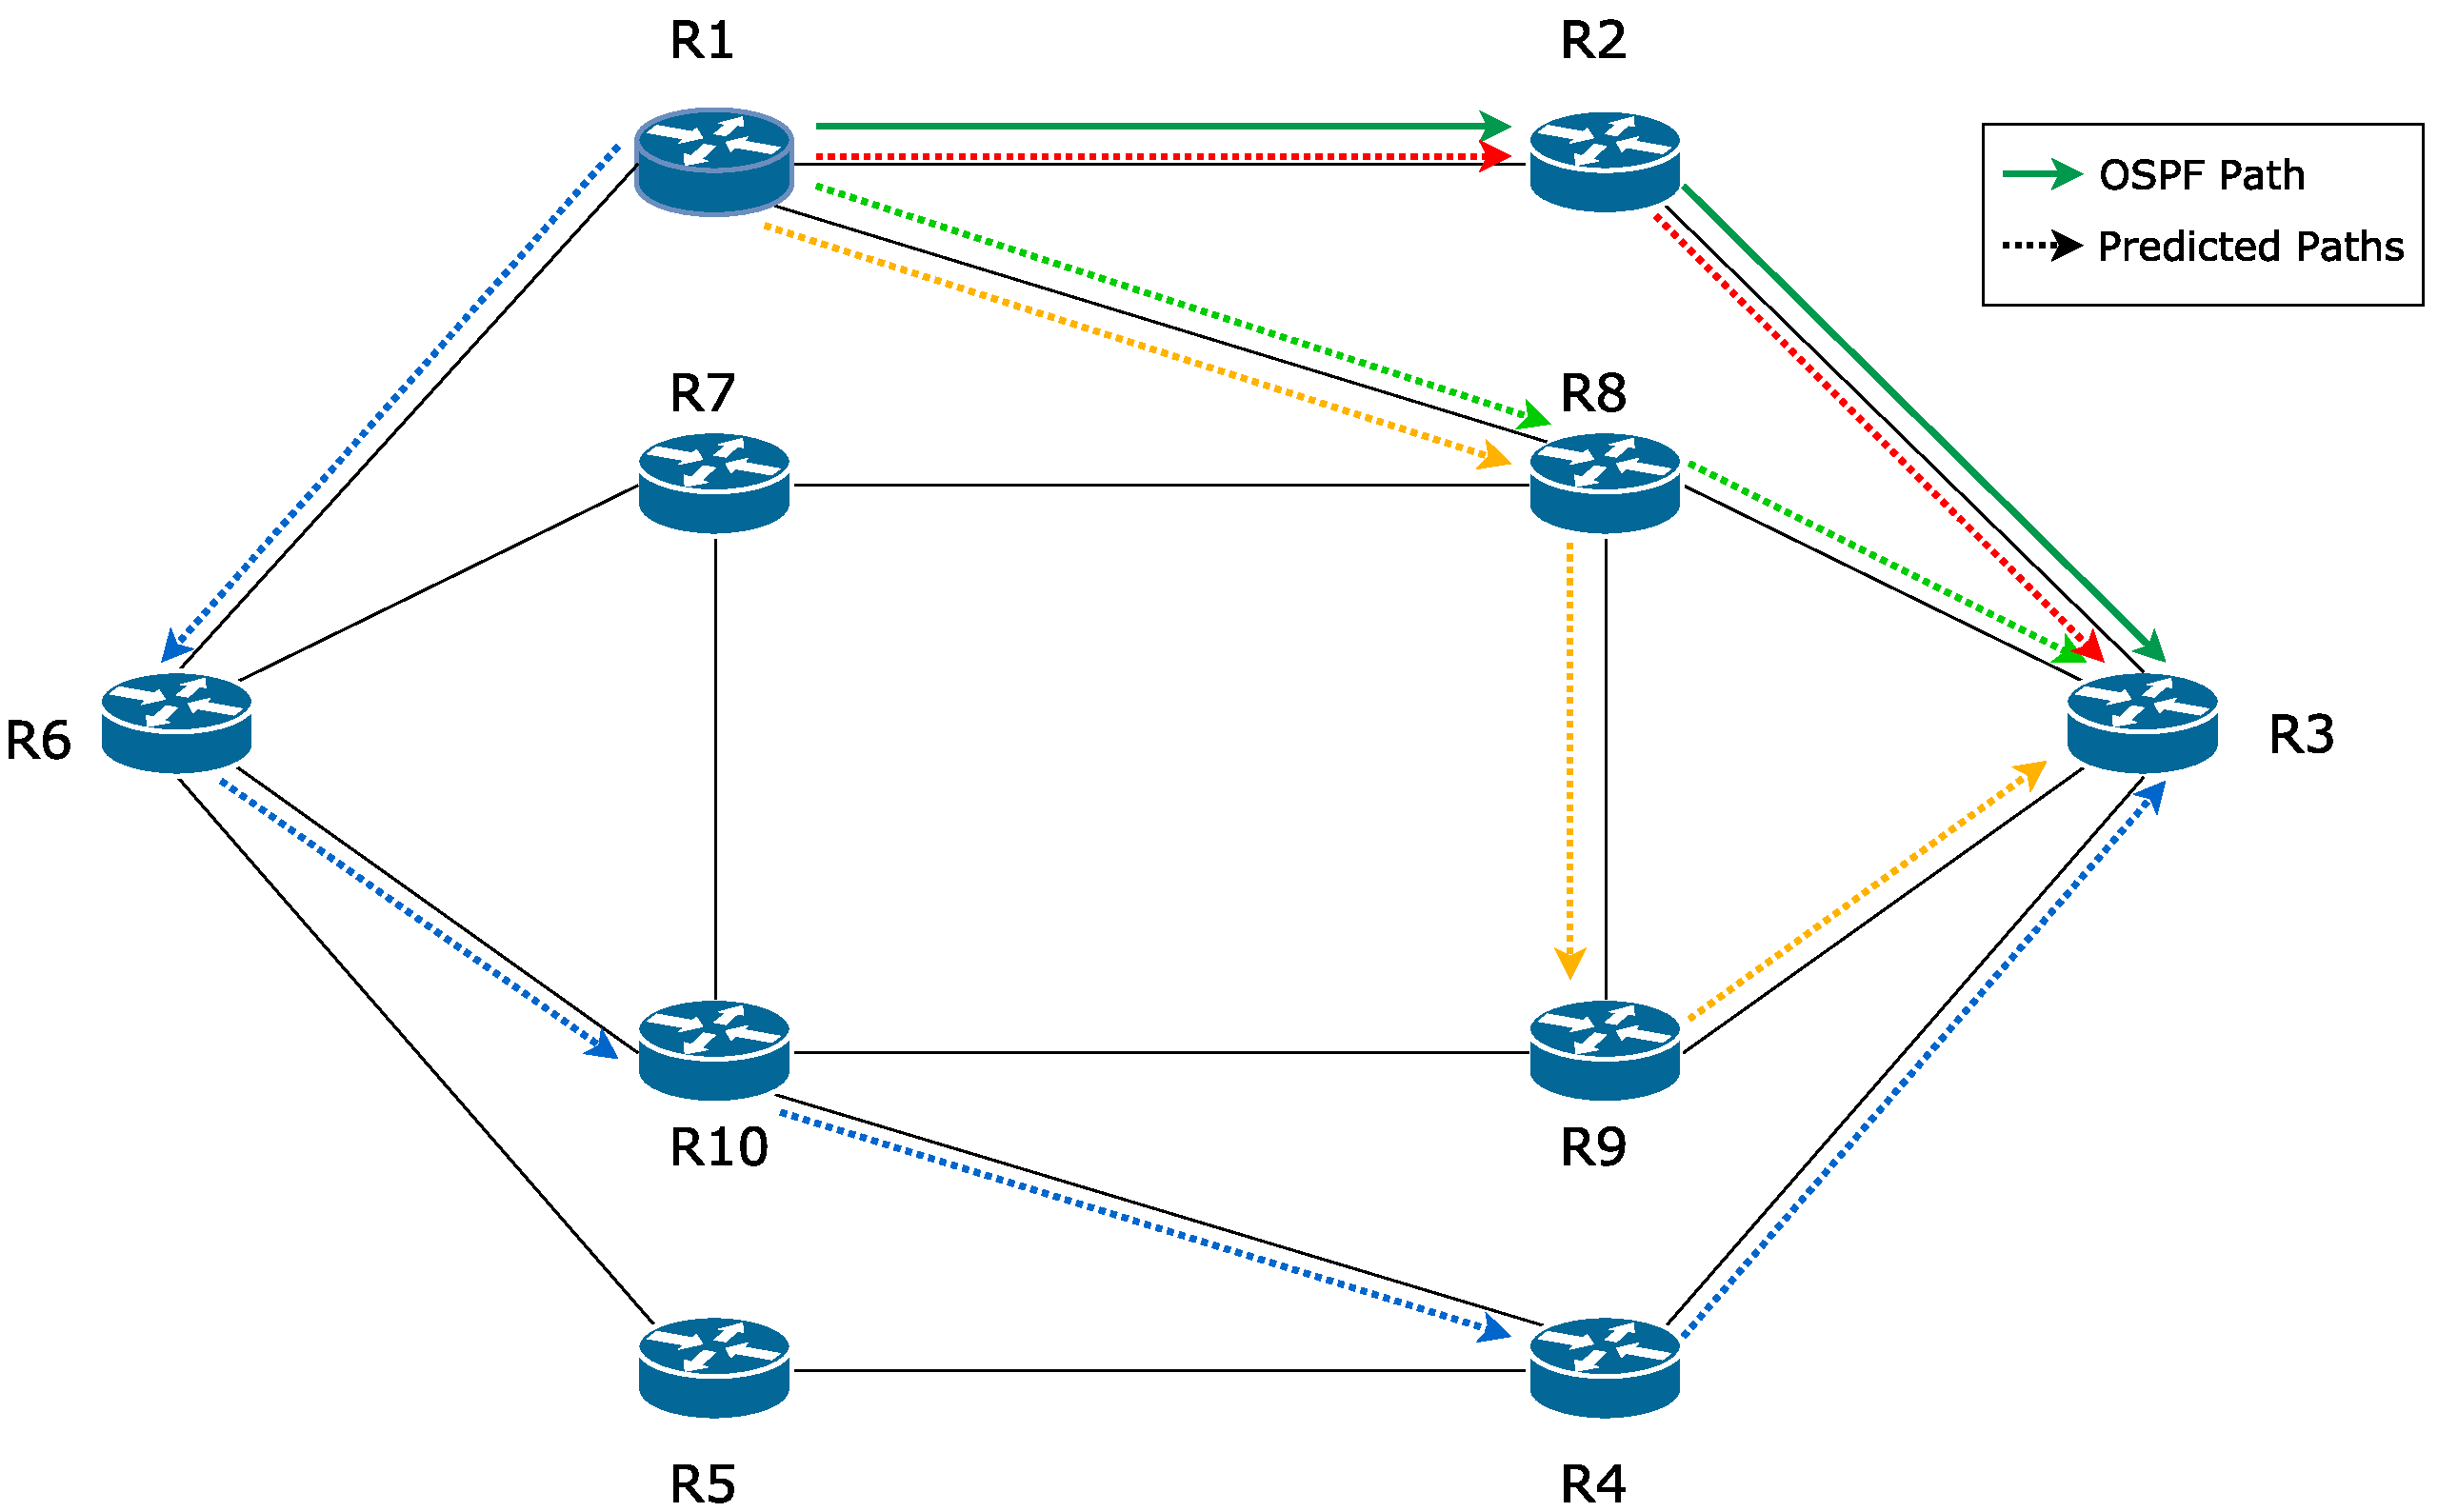
\includegraphics[width=0.85\textwidth]{img/path_comparison}\\
	\flushleft	
	The LSTM path predictor suggests multiple paths
	}

	\frame{\frametitle{LSTMs outrun current approaches in terms of retransmission}
	In case of malfunctioning links, our system has a lower retransmission percentage then traditional routing\\~\\
	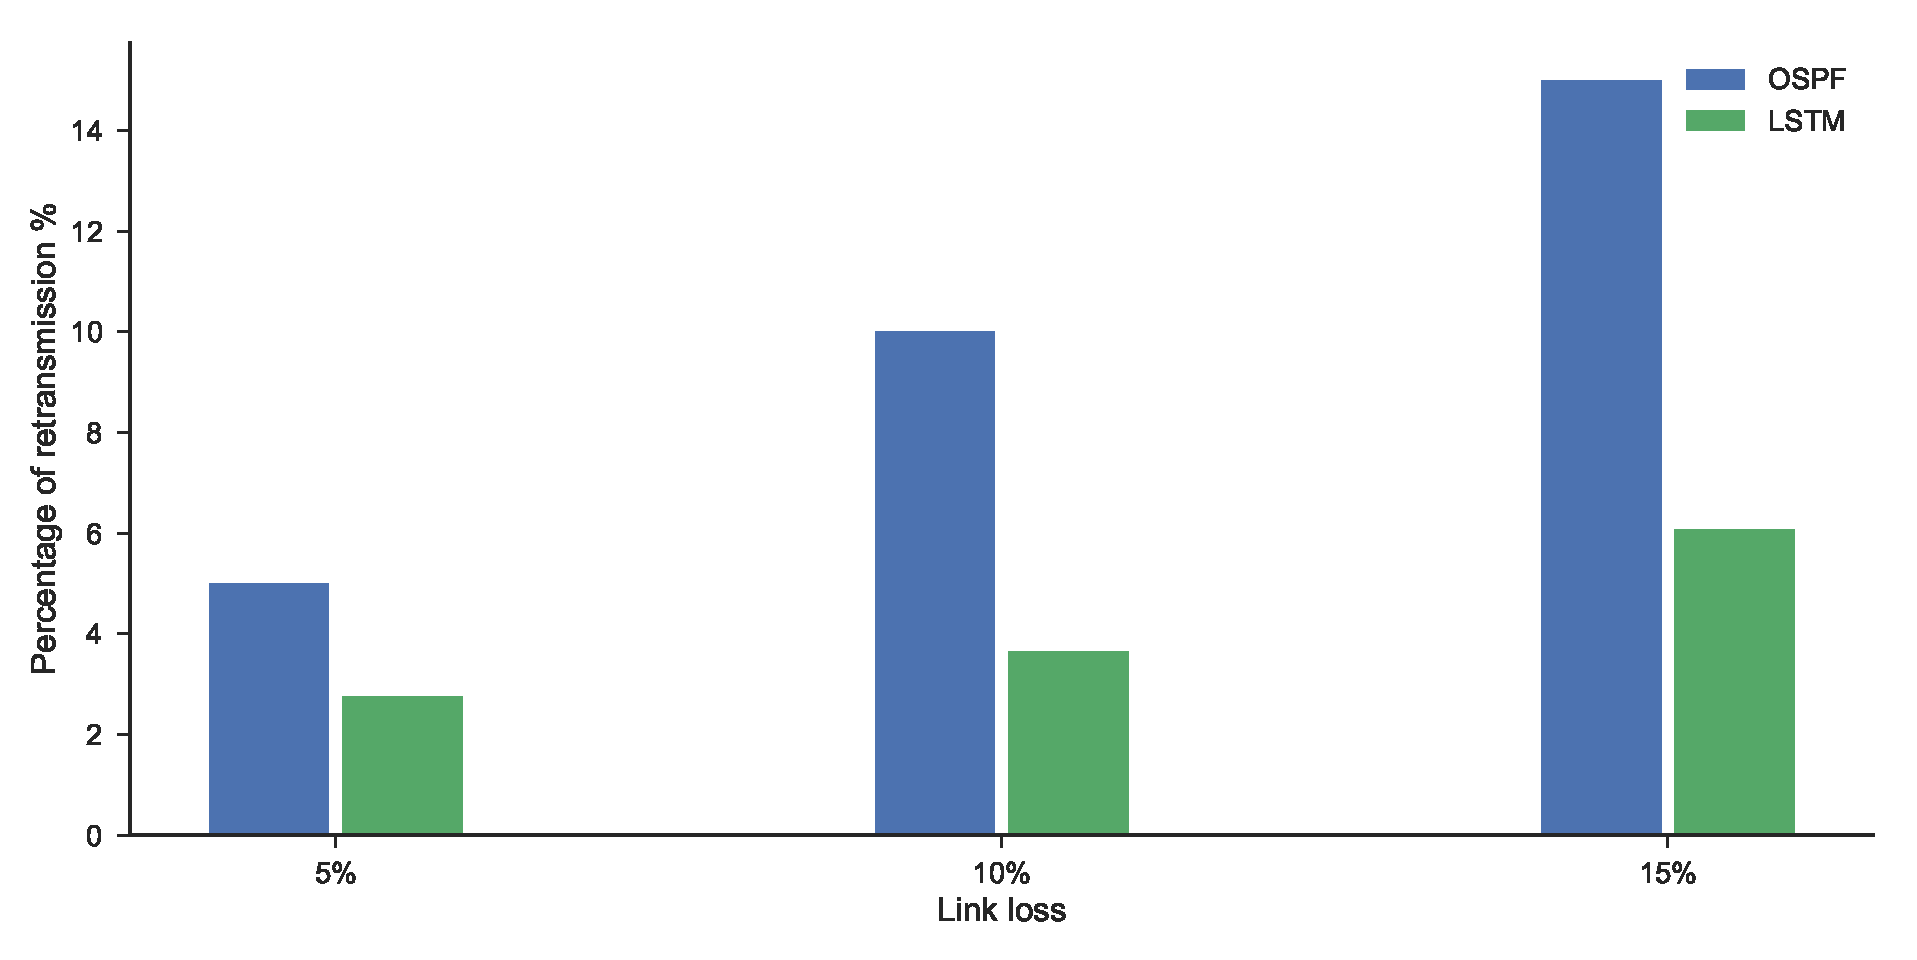
\includegraphics[width=\textwidth]{img/prediction_cmp_bar}\\
	\tiny{\textit{OSPF = Open Shortest-Path First, LSTM = Long Short-Term Memory
}	}}

\section{Future work}
	\mytoc
	
	\frame{\frametitle{Future work}
	Current results are encouraging, therefore  we want to further investigate the problem by:
	\begin{itemize}
	\item getting rid of Mininet emulation environment constraints  
	\item testing the method on larger networks (e.g GENI)
	\item running the testbed on a more scalable platform (e.g GPU)
	\item exploring more machine learning techniques \\(e.g reinforcement learning)
\end{itemize}		
	}
\section*{Take home messages}
\begin{frame}{Take home messages}
\begin{itemize}
\item	Mobile edge computing is a complex problem\\
\pause
\item	We prototyped an architecture for MEC offloading orchestration\\
\pause
\item	We developed a machine learning-based, performance aware routing strategy that improves on classic iBGP mechanisms
\end{itemize}	
\end{frame} 

\begin{frame}[standout]
  \Large An Architecture for Task and Traffic Offloading \\in Edge Computing via Deep Learning\\
    \vspace{1cm}
	\large Thank you for the attention\\  
  \vspace{1cm}
  {\small Alessandro Gaballo}
\end{frame}

%backup slides
\begin{frame}[allowframebreaks, noframenumbering, fragile]{Protocol}
\centering
%\textbf{messages.proto}
\begin{lstlisting}
message OffloadRequest {
    message Requirements {
        enum Latency {
            URGENT = 0;
            STANDARD = 1;
            LOOSE = 2;
        }

        float cpu = 1;
        int32 memory = 2;
        Latency latency = 3;
    }
    
    enum Type {
        LAMBDA = 0;
        STANDARD = 1;
    }

    message Task {
        message TaskWrapper {
            enum WrapperType {
                JAR = 0;
                EGG = 1;
            }

            string name = 1;
            WrapperType type = 2;
            bytes task = 3;
        }

        oneof task_location {
            string task_id = 1;
            TaskWrapper wrapper = 2;
        }
    }




    Requirements requirements = 1;
    Type type = 2;
    Task task = 3;

}

message Response{
    enum Result {
        OK = 0;
        INVALID_MSG_SIZE = 1;
        INVALID_REQUEST = 2;
    }

    Result result = 1;
    string msg = 2;
}

message Message{
    enum Type {
        OFFLOAD_REQUEST = 0;
        RESPONSE = 1;
        TASK = 2;
    }
    
    

    Type type = 1;
    oneof msg_type {
        OffloadRequest off_req = 2;
        OffloadRequest.Task task = 3;
        Response response = 4;
    }
}

\end{lstlisting}
\end{frame}

\begin{frame}[noframenumbering]{Recurrent Neural Network vs Long Short Term Memory}
\centering
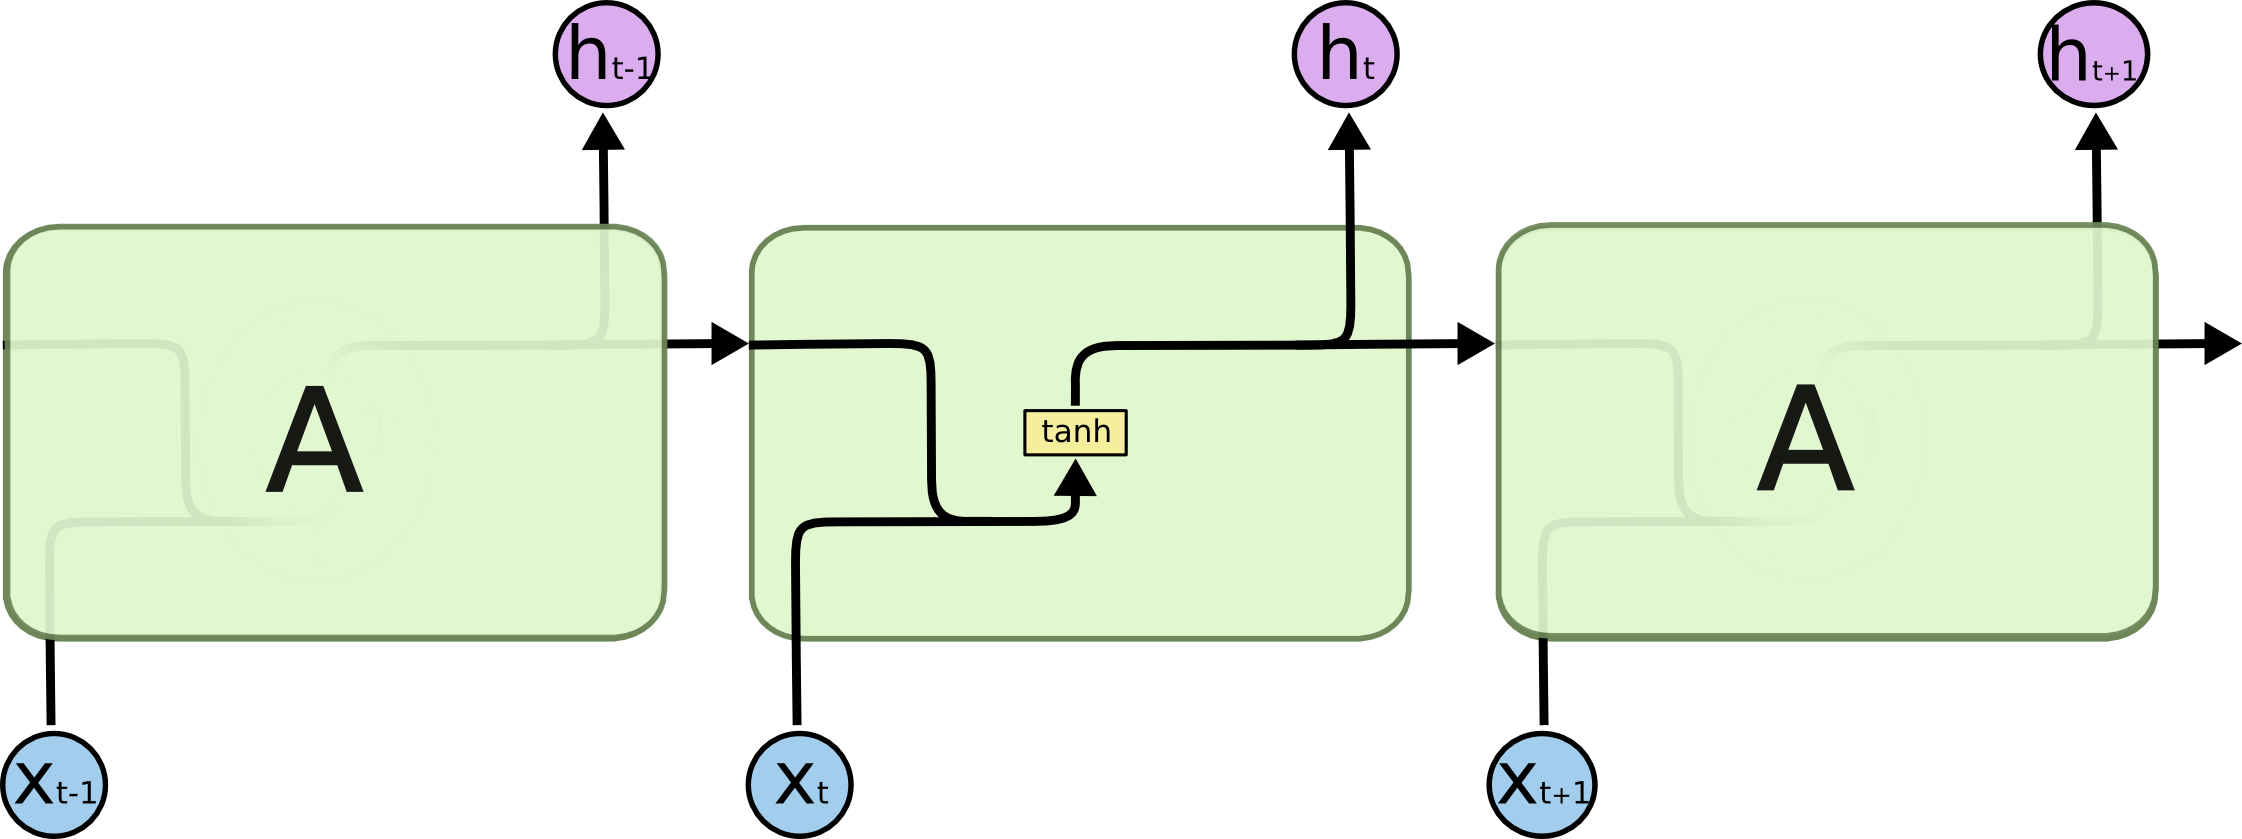
\includegraphics[width=0.8\textwidth]{img/simple_rnn}\\~\\
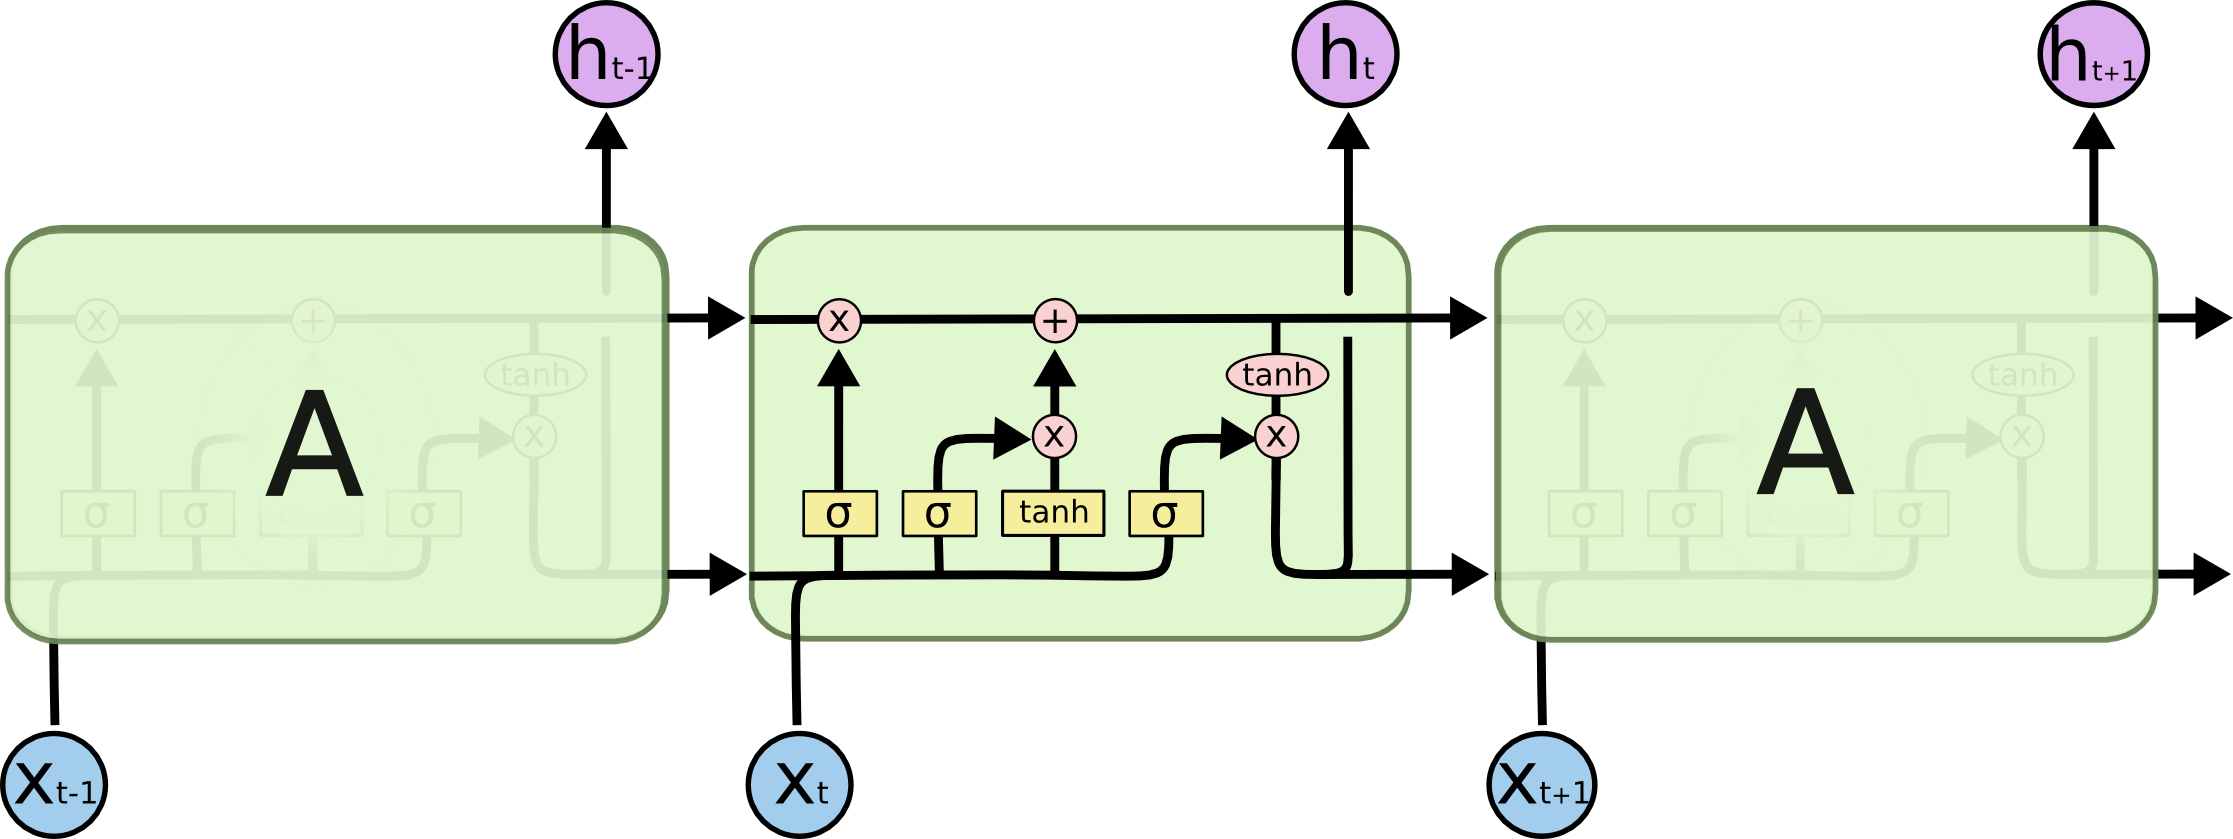
\includegraphics[width=0.8\textwidth]{img/simple_lstm}
\end{frame}
\begin{frame}[noframenumbering]{LSTM cells - activation function}
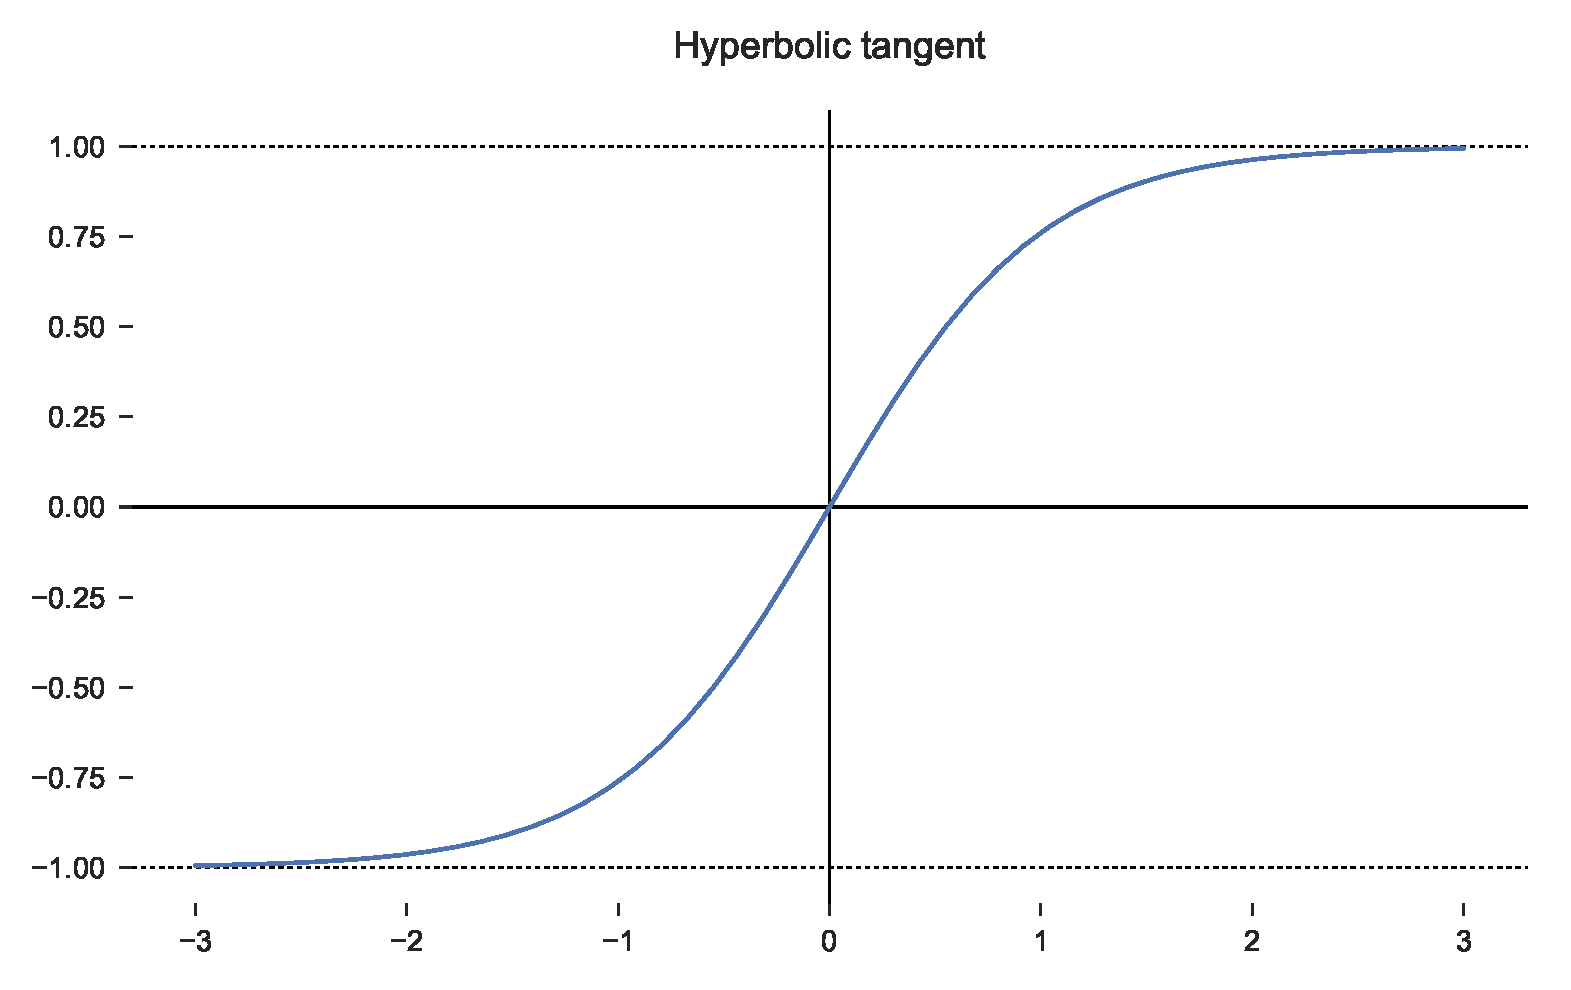
\includegraphics[width=\textwidth]{img/tanh.eps}
\end{frame}
\begin{frame}[noframenumbering]{Comparing with other techniques}
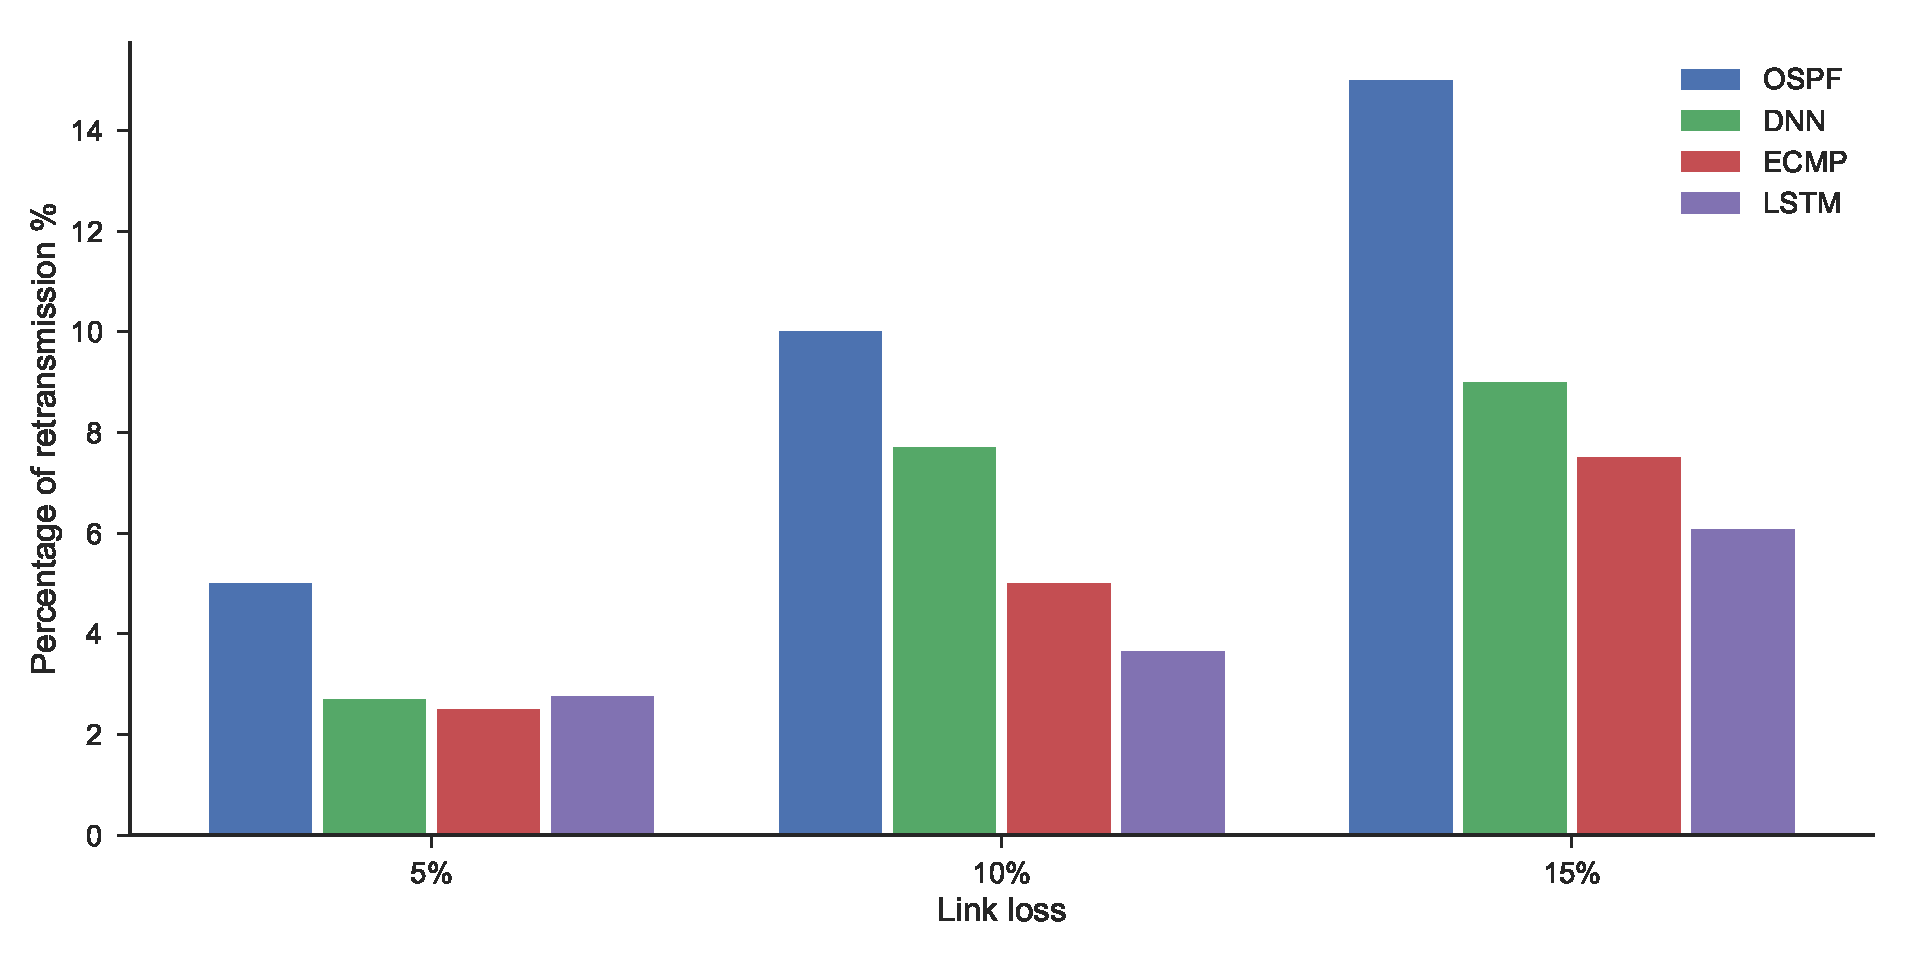
\includegraphics[width=\textwidth]{img/prediction_full_cmp_bar}
\end{frame}
\begin{frame}{Example: computing the path from R1 to R4}	
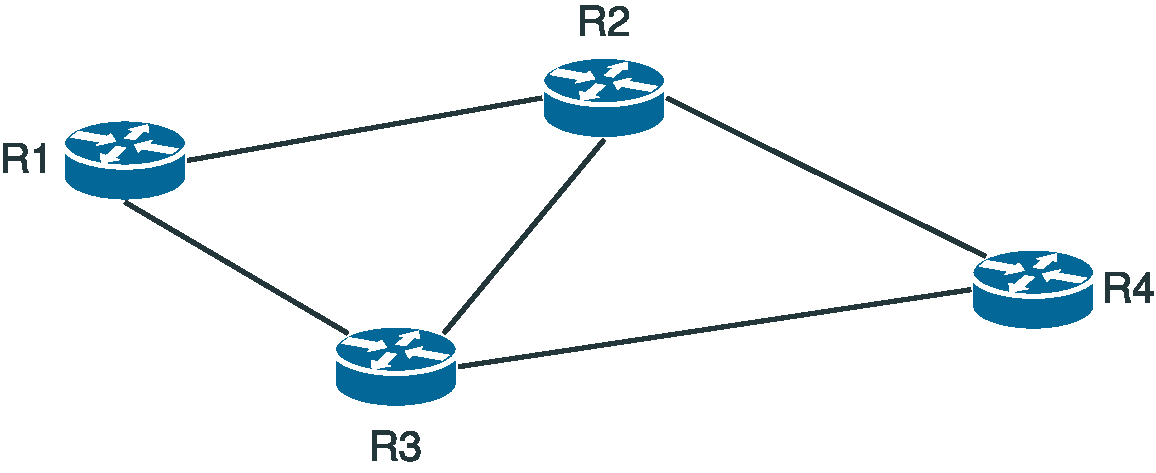
\includegraphics[width=\textwidth]{img/example.pdf}\\
Step 1 - model = R1-R4 --> next hop = R2\\
Step 2 - model = R2-R4 --> next hop = R3\\
Step 3 - model = R3-R4 --> next hop = R4 \\~\\
Computed path: R1 - R2 - R3 - R4\\
\end{frame}
\begin{frame}{Dataset generation}
	To train our model we need:
	\begin{itemize}
	\item network topology
	\item routing algorithm
	\item packet counter
\end{itemize}
	We could not find any public dataset suited to our needs so we create our own.
\end{frame}

\begin{frame}{Network topology}
	We create this topology using MiniNeXt
	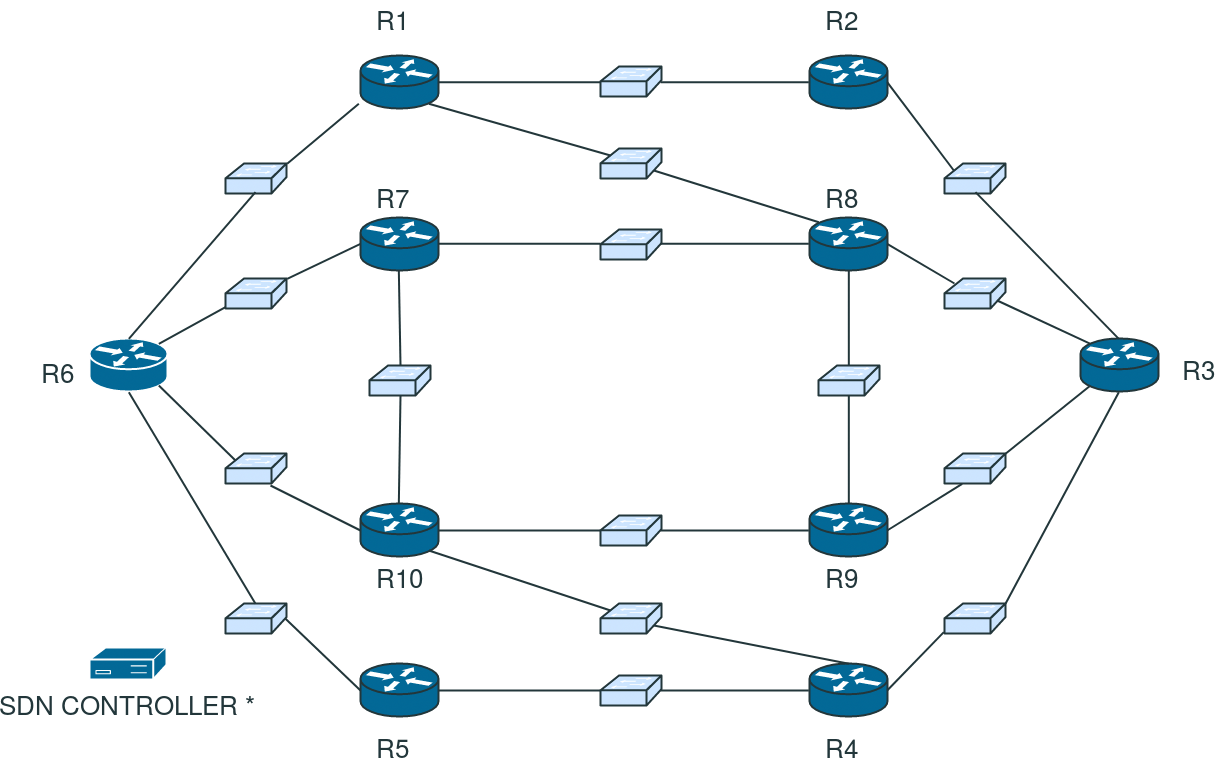
\includegraphics[width=\textwidth]{img/network_arch}\\ 
	\tiny{\textit{* All switches are connected to the SDN controller}}	
\end{frame}
\begin{frame}{Routing algorithm}
	To run routing algorithms on MiniNeXt nodes we use Quagga.\\
	Quagga is a routing suite providing different routing algorithms (e.g OSPF, IS-IS, RIP).\\~\\
	We choose Open Shortest Path First (OSPF) because of its wide adoption as iBGP.\\
\end{frame}
\begin{frame}{Packet counter}
	The SDN controller --Ryu-- is responsible of retrieving the packet count.\\~\\
	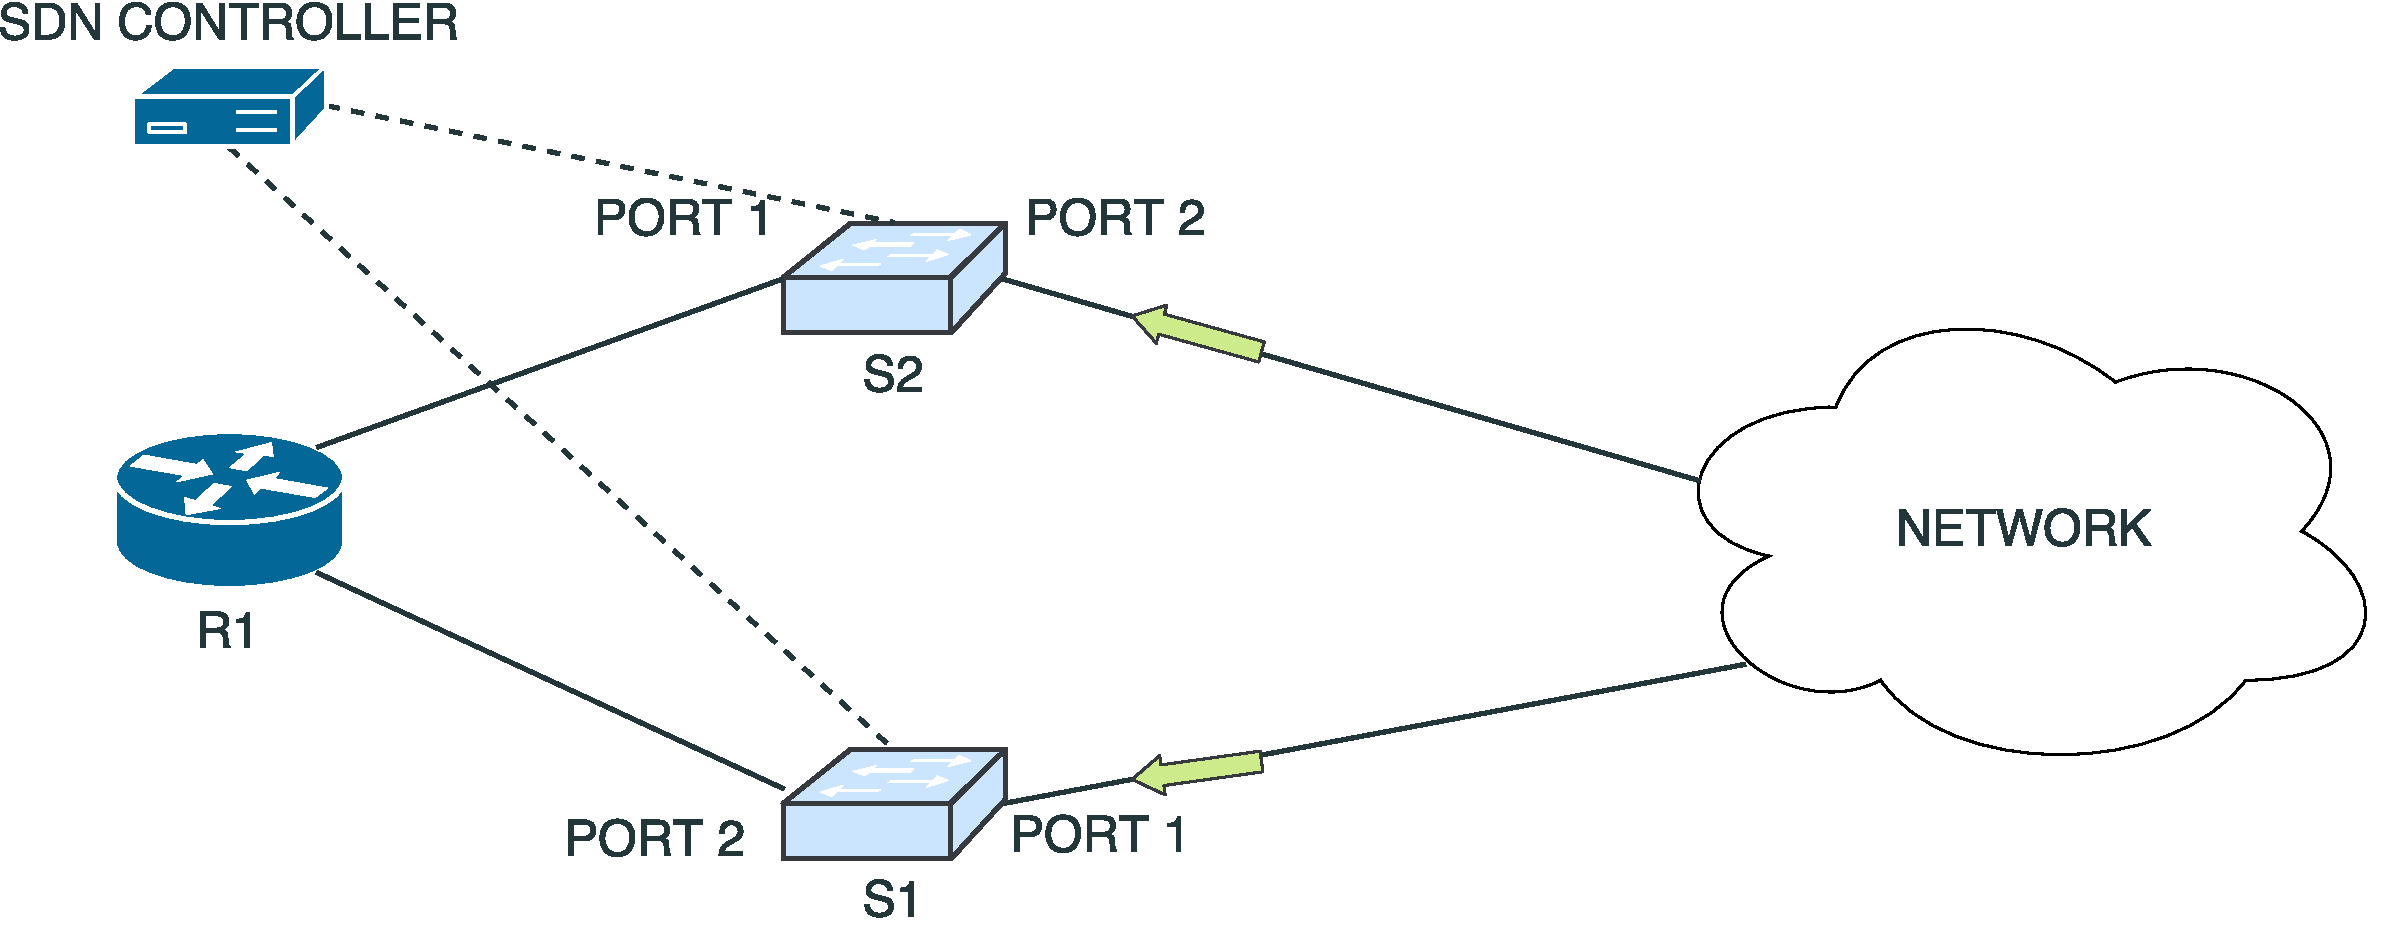
\includegraphics[width=\textwidth]{img/packet_counter.pdf}
\end{frame}
\begin{frame}{Dataset generation steps}
	For an arbitrary number of times:
	\begin{enumerate}
	\item\label{p1} Initialize the topology with different link speed
	\item Simulate traffic between routers
	\item Save packet count and routing tables
	\item Stop the traffic simulation and tear down the network
	\item Back to step~\ref{p1}
	\end{enumerate}
\end{frame}
\begin{frame}{Tuning the network: input normalization}
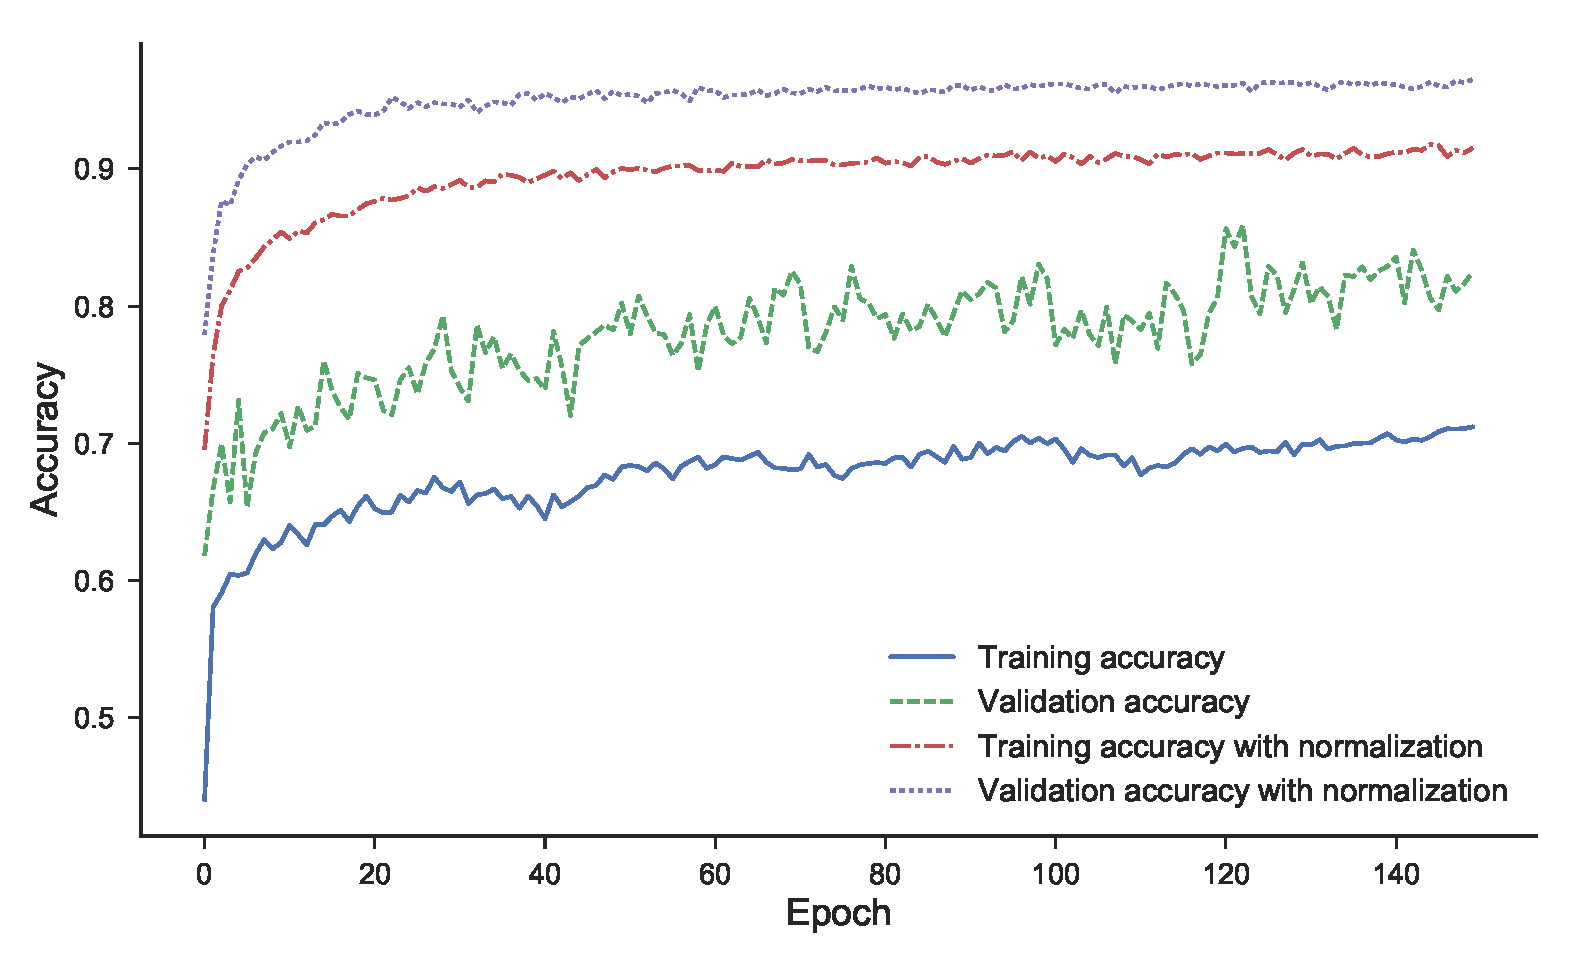
\includegraphics[width=\textwidth]{img/normalization_acc_cmp}	\\~\\
\tiny{\textit{* Accuracy shown only for models with 128 neurons}}	
\end{frame}
	
\begin{frame}{Our prediction model}	
	To use a LSTM we must define the model input and output.\\
	~\\
	\begin{columns}[totalwidth=\textwidth]
	\begin{column}{0.49\textwidth}
	\textbf{Input:}\\~\\
	Incoming packets count \\on each router\\~\\
	\end{column}
	\begin{column}{0.49\textwidth}  %%<--- here
	\textbf{Output:}\\~\\
	One-hot encoded vector \\with the next hop in the path\\~\\
\end{column}
\end{columns}
	\centering
	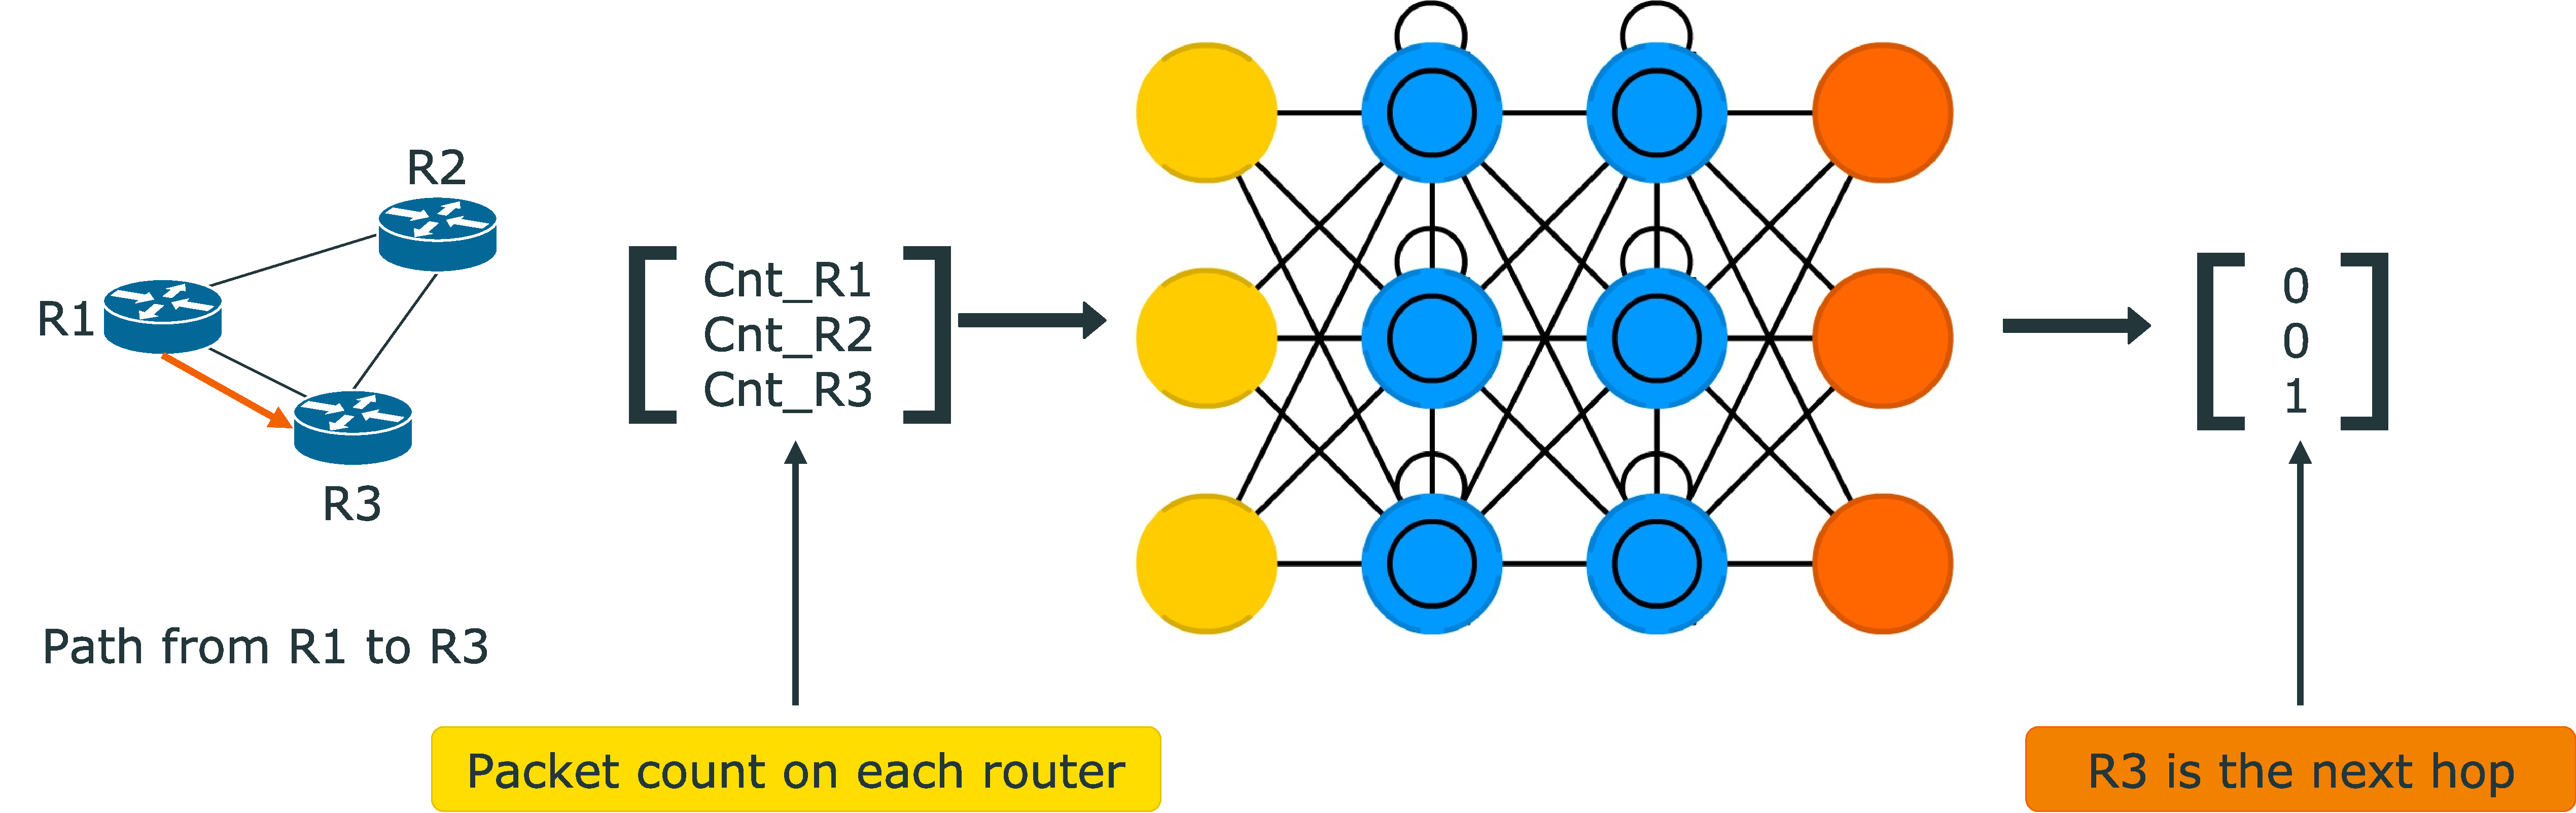
\includegraphics[width=\textwidth]{img/prediction_flow}
\end{frame}
\begin{frame}{Limitations}
	Testbed:
	\begin{itemize}
	\item The functionalities of Mininet are limited
	\item Higher link loss decreases the prediction efficiency
	\end{itemize}
	~\\
	Computation:	
	\begin{itemize}
	\item The number of models to train is big
	\item The trained models occupy GBs of memory
	\end{itemize}
\end{frame}
\end{document}